\documentclass[a4paper, 11pt]{article}
\usepackage[utf8]{inputenc}
\usepackage[czech]{babel}
\usepackage{times}
\usepackage[left=2cm, text={17cm, 24cm}, top=3cm]{geometry}
\usepackage{multirow}
\usepackage[ruled,longend,linesnumbered,noline]{algorithm2e}
\usepackage{graphicx}
\usepackage{pdflscape}

\newcommand{\uvcs}[1]{\quotedblbase #1\textquotedblleft}

\begin{document}
\begin{titlepage}
    \begin{center}
        {\Huge\textsc{Vysoké učení technické v~Brně}}\\[0.4em]
        {\huge\textsc{Fakulta informačních technologií}}
        
    
    \vspace{\stretch{0.4}}
    
    {\LARGE 
        Typografie a publikování\,--\,3. projekt}\\[0.3em]
        {\Huge Tabulky a obrázky}
    
    \vspace{\stretch{0.5}}
    \end{center}
    
    {\Large 24.marca 2021 \hfill Igor Hanus (xhanus19)} 
    
\end{titlepage}




\section{Úvodní strana}
Název práce umístěte do zlatého řezu a nezapomeňte uvést dněšní dátum a vaše jméno a příjmení.

\section{Tabulky}
Pro sázení tabulek můžeme použít buď prostředí \verb|tabbing| nebo prostředí \verb|tabular|

\subsection{Prostředí \texttt{tabbing}}
Při použití \texttt{tabbing} vypadá tabulka nasledovně:

\begin{tabbing}
\hspace*{2.8cm}\=\hspace*{1.4cm}\=\hspace*{2cm}\kill
\textbf{Ovoce} \> \textbf{Cena} \> \textbf{Množství}\\
Jablka \> 25,90\>3 kg \\
Hrušky \> 27,40\>2,5 kg \\
Vodní melouny \> 35,-\>1 kus \\
\end{tabbing}
Toto prostředí se dá také použít pro sázení algoritmů, ovšem vhodnejší použít prostředí \texttt{algorithm} nebo \texttt{algorithm2e} (viz sekce \ref{section:Algorithms}).

\subsection{Prostředí \texttt{tabular}}
Další možností, jak vytvořit tabulku, je použít prostředí \texttt{tabular.} Tabulky pas budou vypadat takto\footnote{Kdyby byl problem s~\texttt{cline}, zkuste se podívat třeba sem:  http://www.abclinuxu.cz/tex/poradna/show/325037.}:

\bigskip
\catcode`\-=12
\begin{table}[h]
    \centering
\begin{tabular}{ | c | c | c |}
    \hline
                  & \multicolumn{2}{|c|}{\textbf{Cena}} \\ \cline{2-3}
    \textbf{Měna} & \textbf{nákup}   &   \textbf{prodej}\\ \hline
    EUR          & 25,277           & 26,943           \\
    GBP          & 29,368           & 31,492           \\
    USD          & 21,260           & 22,661           \\ \hline
    
\end{tabular}
\caption{Tabulka kurzů k dnešnímu dni}
\label{tables:table1}
\end{table}

\bigskip
\catcode`\-=12
\begin{table}[h]
    \centering
    
\begin{tabular}{ | c | c | }
    \hline
    $A$ & $\neg A$\\ \hline
    \textbf{P}          & N  \\ \hline
    \textbf{O}          & O  \\ \hline
    \textbf{X}          & X  \\ \hline
    \textbf{N}          & P  \\ \hline
    
\end{tabular}
\begin{tabular}{|c|c|c|c|c|c|}
\hline
\multicolumn{2}{|l|}{         \multirow{2}{*}{$A \wedge B$}} & \multicolumn{4}{c|}{$B$}    \\ \cline{3-6} 
\multicolumn{2}{|l|}{}      & \textbf{P}    & \textbf{O}   & \textbf{X}   & \textbf{N}   \\ \hline
\multirow{4}{*}{$A$}        & \textbf{P}    & P            & O            & X      & N   \\ \cline{2-6} 
                            & \textbf{O}    & O            & O            & N      & N   \\ \cline{2-6} 
                            & \textbf{X}    & X            & N            & X      & N   \\ \cline{2-6} 
                            & \textbf{N}    & N            & N            & N      & N   \\ \hline
\end{tabular}
\begin{tabular}{|c|c|c|c|c|c|}
\hline
\multicolumn{2}{|l|}{         \multirow{2}{*}{$A \vee B$}} & \multicolumn{4}{c|}{$B$}    \\ \cline{3-6} 
\multicolumn{2}{|l|}{}      & \textbf{P}    & \textbf{O}   & \textbf{X}   & \textbf{N}   \\ \hline
\multirow{4}{*}{$A$}        & \textbf{P}    & P            & P            & P      & P   \\ \cline{2-6} 
                            & \textbf{O}    & P            & O            & P      & O   \\ \cline{2-6} 
                            & \textbf{X}    & P            & P            & X      & X   \\ \cline{2-6} 
                            & \textbf{N}    & P            & O            & X      & N   \\ \hline
\end{tabular}
\begin{tabular}{|c|c|c|c|c|c|}
\hline
\multicolumn{2}{|l|}{         \multirow{2}{*}{$A \rightarrow B$}} & \multicolumn{4}{c|}{$B$}    \\ \cline{3-6} 
\multicolumn{2}{|l|}{}      & \textbf{P}    & \textbf{O}   & \textbf{X}   & \textbf{N}   \\ \hline
\multirow{4}{*}{$A$}        & \textbf{P}    & P            & O            & X      & N   \\ \cline{2-6} 
                            & \textbf{O}    & P            & O            & P      & O   \\ \cline{2-6} 
                            & \textbf{X}    & P            & P            & X      & X   \\ \cline{2-6} 
                            & \textbf{N}    & P            & P            & P      & P   \\ \hline
\end{tabular}
\caption{Protože Kleeneho trojhodnotová logika už je \uvcs{zastaralá}, uvádíme si zde příklad čtyřhodnotové logiky}
\label{tables:table2}
\end{table}

\section{Algoritmy} \label{section:Algorithms}
Pokud budeme chtít vysázet algoritmus, můžeme použít prostředí {\texttt{algorithm}\footnote{Pro nápovědu, jak zacházet s~prostředím \texttt{algorithm}, můžeme zkusit stránku: \\ http://ftp.cstug.cz/pub/tex/CTAN/macros/latex/contrib/algorithms/algorithms.pdf.} }
nebo\,
\texttt{algorithm2e}\footnote{Pro \texttt{algorithm2e} zase tuhle: http://ftp.cstug.cz/pub/tex/CTAN/macros/latex/contrib/algorithm2e/doc/algorithm2e.pdf}.
Příklad použití prostředí \texttt{algorithm2e} viz Algoritmus \ref{algorithms:algorithm1}.
\bigskip

\IncMargin{1.5 em}
\begin{algorithm} 
\SetNlSty{}{}{:}

\Indm
\KwIn{$X_{t-1}, u_t, z_t)$}
\KwOut{$X_t$}
\BlankLine

\Indp
$\overline{X_t} = X_t = 0 $ \\
\For{$ k = 1 \emph{ to } M $} {
    \Indpp
    $x^{[k]}_t = \emph{sample\_motion\_model} (u_t,x^{[k]}_{t-1})$ \\
    $\omega^{[k]}_t = \emph{measurement\_model} (z_t,x^{[k]}_t,m_{t-1})$ \\
    $m^{[k]}_t = \emph{updated\_occupancy\_grid} (z_t,x^{[k]}_t,m^{[k]}_{t-1})$ \\
    $\overline{X_t} = \overline{X_t} + \langle x^{[m]}_x,\omega^{[m]}_t \rangle $
}
\For{$ k = 1 \emph{ to } M $} {
    \Indpp
    draw \emph{i} with probability $\approx \omega^{[i]}_t$ \\
    add $\langle x^{[k]}_x,m^{[k]}_t\rangle$ to $X_t$
}
\KwRet{$X_t$}
\caption{\textsc{FastSLAM}}
\label{algorithms:algorithm1}
\end{algorithm}
\DecMargin{1.5 em}

\section{Obrázky}
Do našich článků můžeme samozřejmě vkládat obrázky. Pokud je obrázkem fotografie,
můžeme klidně použít bitmapový soubor. Pokud by to ale mělo být nějaké schéma nebo
něco podobného, je dobrým zvykem takovýto obrázek vytvořit vektorově.
    
    \begin{figure}[h] 
       \centering
       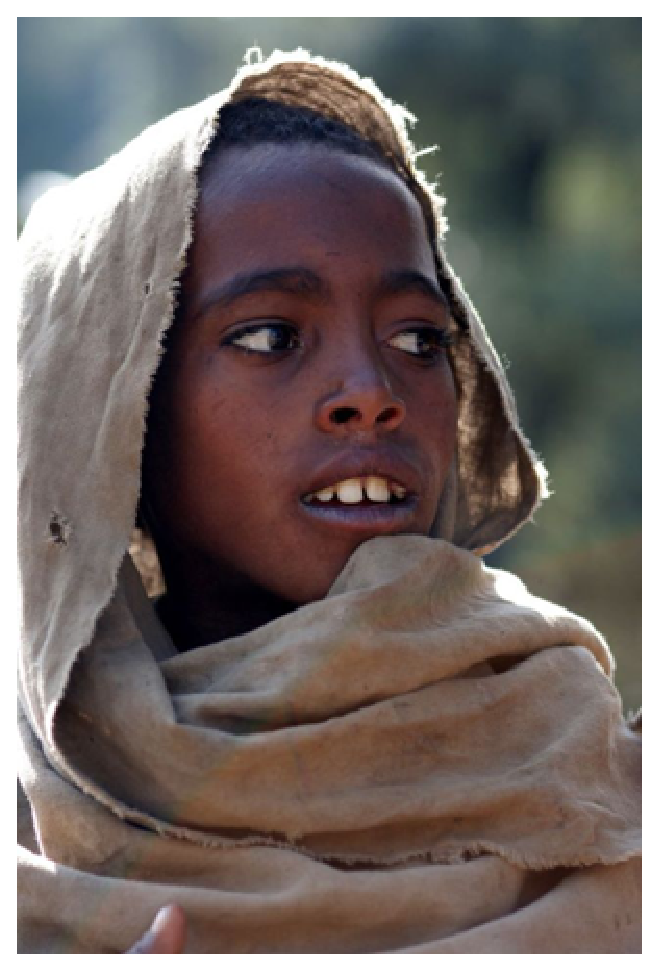
\includegraphics[scale=0.4]{etiopan.eps}
       \hspace{-0.16cm}
       \scalebox{-1}[1]{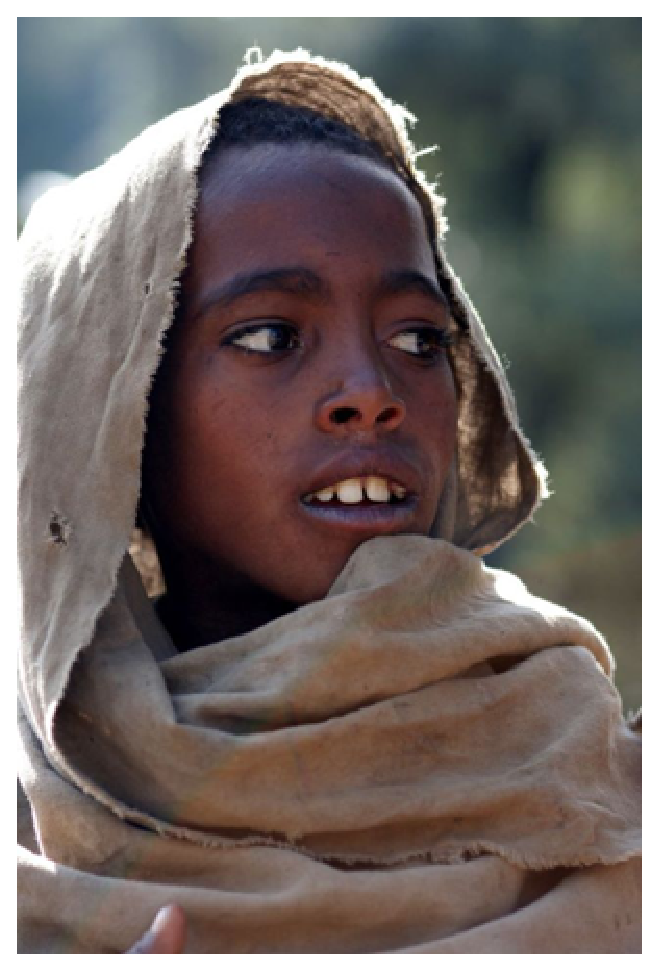
\includegraphics[scale=0.4]{etiopan.eps}}
       \caption{Malý Etiopánek a jeho bratříček}
       \label{images:image1}
    \end{figure}
Rozdíl medzi vektorovým\dots

\begin{figure}[h] 
   \centering
   
\includegraphics[scale=0.4]{oniisan.eps}
   \caption{Vektorový obrázek}
   \label{images:image2}
\end{figure}

\noindent\dots a bitmapovým obrázkem

\begin{figure}[h] 
   \centering
   
\includegraphics[scale=0.6]{oniisan2.eps}
   \caption{Bitmapový obrázek}
   \label{images:image3}
\end{figure}

\noindent se projeví například při zvětšení.

Odkazy (nejen ty) na obrázky \ref{images:image1}, \ref{images:image2} a \ref{images:image3}, na tabulky \ref{tables:table1} a \ref{tables:table2} a také na algoritmus \ref{algorithms:algorithm1} jsou udělany pomocí křížových odkazů. Pak ovšem potřeba zdrojový soubor přeložit dvakrát.

Vektorové obrázky lze vytvořit i přímo v \LaTeX u, například pomocí prostředí \texttt{picture}.
\newpage

\begin{landscape}
		\begin{figure}[h]
			\setlength{\unitlength}{1mm}
			\centering
			\begin{picture}(200, 120)
				\linethickness{1pt}
				\put(0, 0){\framebox(220, 120){}}
				
				\linethickness{5pt}
				\put(5, 10){\line(1, 0){210}}
				
				\linethickness{1pt}
				\put(30,10){\line(0,1){45}}
				\put(30,55){\line(1,0){60}}
				\put(90,47){\line(0,1){12}}
				\put(90,59){\line(1,0){60}}
				\put(45,47){\line(1,0){150}}
				\put(150,59){\line(0,-1){12}}
				\put(195,47){\line(0,-1){8}}
				
				\put(195,39){\line(-1,0){150}}
				\put(45,39){\line(0,1){8}}
				\put(150,49){\line(1,0){40}}
				\put(190,49){\line(0,-1){2}}
				
				\put(40,10){\line(0,1){15}}
				\put(40,25){\line(1,0){30}}
				
				\put(70,25){\line(5,-2){35}}
				\put(45,39){\line(5,-4){17.5}}
				
				\put(190,35){\line(0,-1){15}}
			    \put(190,35){\line(-1,0){115}}
				\put(75,35){\line(0,-1){12}}
				
				\put(190,20){\line(-1,0){107.5}}
				\put(190,20){\line(1,0){5}}
				\put(195,20){\line(0,-1){10}}
				
				\put(190,100){\circle{14}}
				\put(183,107){\line(1,0){15}}
				\put(187,107){\line(0,1){7}}
				\put(194,107){\line(0,1){7}}
				\put(187,114){\line(1,0){7}}
				
				\linethickness{4pt}
				\put(187,109){\line(1,0){7}}
				
			\end{picture}
			\caption{Vektorový obrázek moderního domu se slunkem s kloboukem.}
			\label{images:image4}
		\end{figure}
	\end{landscape}

\end{document}
